% Created 2018-02-08 Thu 15:58
\documentclass[11pt]{article}
\usepackage[utf8]{inputenc}
\usepackage[T1]{fontenc}
\usepackage{fixltx2e}
\usepackage{graphicx}
\usepackage{longtable}
\usepackage{float}
\usepackage{wrapfig}
\usepackage{rotating}
\usepackage[normalem]{ulem}
\usepackage{amsmath}
\usepackage{textcomp}
\usepackage{marvosym}
\usepackage{wasysym}
\usepackage{amssymb}
\usepackage{hyperref}
\tolerance=1000
\date{\today}
\title{WorldCiv}
\hypersetup{
  pdfkeywords={},
  pdfsubject={},
  pdfcreator={Emacs 25.3.1 (Org mode 8.2.10)}}
\begin{document}

\maketitle
\tableofcontents

\section{History 1310 - Science and Technology in World Civilization}
\label{sec-1}

Date: \textit{<2018-01-18 Thu>} Lecturer: Driggers

\subsection{Questions? :email: edriggers@tntech.edu \textbf{Office Hours}:}
\label{sec-1-1}
T-Th: 4:30-6
What are office hours for? 
\begin{itemize}
\item Problems reading and retaining information from lecture or textbook.

\item Questions about grades, performance, participation, attendance, Etc

\item Go over a test or paper

\item Recommendations about improvement
\end{itemize}

\section{Lecture 1 - What is the meaning of Science?}
\label{sec-2}

\begin{itemize}
\item Whare is the use of science?

\item Are there ways that science can be improperly?

\item Is science value free?

\item How do non-epistimic values figure into scientific investigations?

\item What are the role of

\item contextual values in science?

\item Whose values will impact scientific work?
\end{itemize}

\subsection{What do I mean by Values???}
\label{sec-2-1}

\begin{itemize}
\item Epistimic-Traditionally means values in the internal processes of science? 
Like measurement, quantification, ?Testable?

\item Non-Epistimic-Means those not in the internal process, often effecting the conceptualization of questions and interpretation of ?data,? things like experiences, psychological worries, political values, ideas about race, gender \&c.

\item Objectivity is a changing standard throughout history!
\end{itemize}


\subsection{Traditional Conception of Scientific Investigation}
\label{sec-2-2}
\begin{itemize}
\item Scientists:

\begin{itemize}
\item Observe phenomena, Measure it, and Understand and make products; control phenomena; offer recommendations
\end{itemize}

\item Who are scientists?

\item What is deemed phenomena?

\item What counts as proper measurement?

\item Why are conclusions drawn, verified, and communicated to professionals and the public(s)?

\item Is science objective? 

\begin{itemize}
\item What questions are we as society comfortable with asking?

\item What is the role of ethics in scientific investigations?
\end{itemize}
\end{itemize}

\subsubsection{Nazi Medical Experimentation and the body}
\label{sec-2-2-1}

\begin{itemize}
\item Examples include, but not limited to: 

\begin{itemize}
\item High Altitude experiments

\item Drug experiments

\item Freezing water
\end{itemize}
\end{itemize}

\subsubsection{Drug Testing and Children}
\label{sec-2-2-2}

\begin{itemize}
\item Case of anti-depressants and adolescents
\end{itemize}



\begin{itemize}
\item Re-branding of drugs for profit * Arthritis \#\#
\end{itemize}

\subsubsection{Conception and understanding of life}
\label{sec-2-2-3}

\begin{itemize}
\item The "Sperm and Egg" Model Traditionally the woman's reproductive system was considered pretty passive, no we know that isn't the case. The woman's body is responsible for "weeding out" the weak of the Man's sperm
\end{itemize}

\subsubsection{Interventions in the environment}
\label{sec-2-2-4}

+Iron sulfate (Fertilizer) dumping into ocean

\section{Lecture 2 - Babylon and beyond}
\label{sec-3}
:Lecturer: Driggers
:DATE: \textit{<2018-01-23 Tue>}

\subsection{Orientation:}
\label{sec-3-1}
\begin{itemize}
\item Survey of history if science, technology, medicine, etc. throughout greater Mesopotamian history
\item General Details, geography, Etc.
\end{itemize}

\subsection{{\bfseries\sffamily TODO} Theoretical Point: \emph{Verify quotes\ldots{}}}
\label{sec-3-2}
\begin{itemize}
\item where SHOULD we start this class?
\texttt{Most professors start much later, with the Greeks; look at history through their eyes}

\item The power of narrative

\item Keep Reading!

\item Problem with Near Eastern Studies - Far East Studies???
To have a proper \emph{Near east study} you have to be \emph{near east}, most aren't.
\end{itemize}

\subsection{Geographic location:}
\label{sec-3-3}
\begin{figure}[htb]
\centering
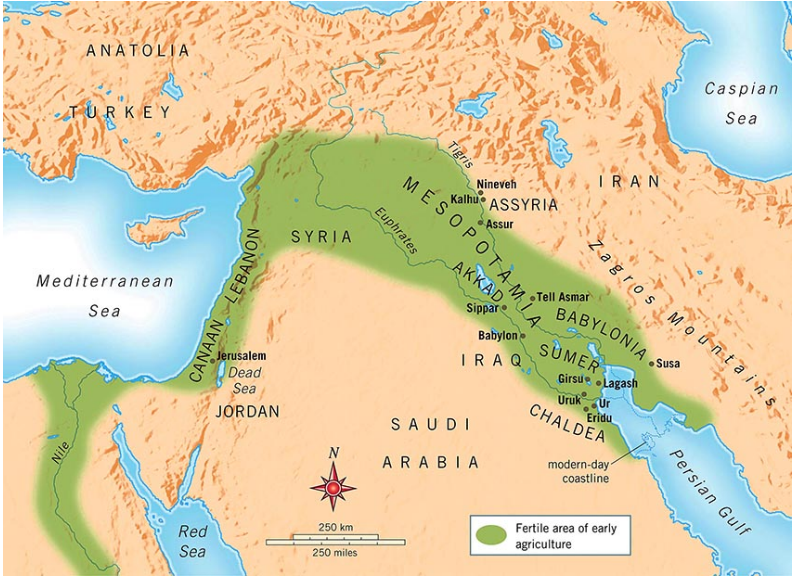
\includegraphics[width=.9\linewidth]{./img/fertileCrescent.png}
\caption{Fertile Crescent of early agriculture}
\end{figure}

\begin{itemize}
\item Framed in Today's Geopolitical Landscape
\end{itemize}
\begin{figure}[htb]
\centering
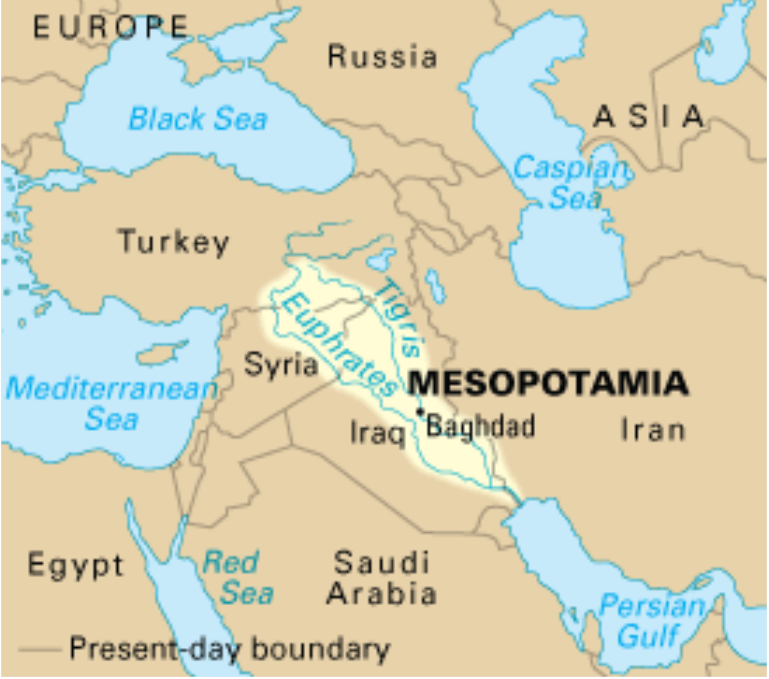
\includegraphics[width=.9\linewidth]{./img/GeoLand.png}
\caption{More modern representation of area.}
\end{figure}

\subsection{Home to diverse groups of people}
\label{sec-3-4}
\begin{itemize}
\item Sumerians

\item Akkadians

\item Persians

\item Babylonians

\item \textbf{Some of the oldest societies}
\end{itemize}

\subsection{Hammurabi and his Code}
\label{sec-3-5}
\begin{itemize}
\item If any one finds runaway male or female slaves in the open country and bring them to their masters, the master of the slaves shall pay him two shekels of silver.

\item If any one is committing a robbery and is caught, then he shall be put to death.

\item If a tavern-keeper (feminine) does not accept corn according to gross weight in payment of a drink, but takes money, and the price of the drink is less than that of the corn, she shall be convicted and thrown into the water.

\item If a son strike his father, his hands be hewn off.

\item If a man knock out the teeth if his equal, his teeth shall be knocked out.

\item If a barber, without the knowledge of his master, but the sign of a slave on a slave not to be sold, the hands of the barber shall be cut off.

\item If a slave says to his master: "You are not my master" - if they convict him his master shall cut off his ear.
\end{itemize}

\subsection{Timeline}
\label{sec-3-6}
\begin{itemize}
\item Goes back to 3500 BC

\item Civilization arose around present day Iraq

\item Communicated throughout a written language: cuneiform
\end{itemize}
\begin{figure}[htb]
\centering
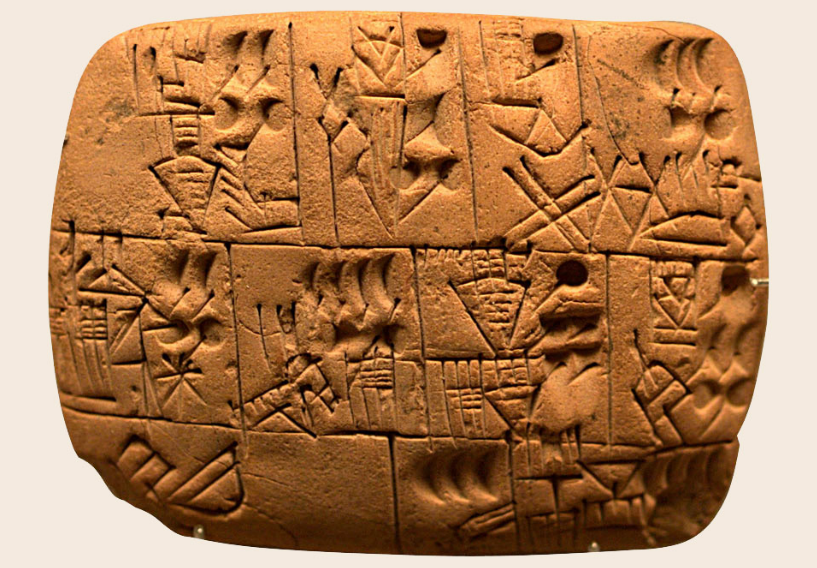
\includegraphics[width=.9\linewidth]{./img/CuneiformTablet.png}
\caption{Cuneiform tablet writing}
\end{figure}

\subsection{Literature: \emph{The Epic of Gilgamesh}}
\label{sec-3-7}
\begin{itemize}
\item Written around 2100 BC

\item About 12 books, or about 5 epic poems

\item \texttt{He saw the Secret, discovered the Hidden, he brought information of (the time) before the Flood. He went on a distance journey, pushing himself to exhaustion, but then was brought peace} (1.5-8)
\end{itemize}

\subsection{Technological Achievement}
\label{sec-3-8}
\begin{itemize}
\item Metalworking (Bronze, Copper, Gold, and eventually iron)

\item Glass making

\item Textile Weaving

\item Water Storage/control
\end{itemize}

\subsubsection{Walls of Babylon \emph{Part of \textbf{Seven Wonder}}}
\label{sec-3-8-1}
\begin{figure}[htb]
\centering
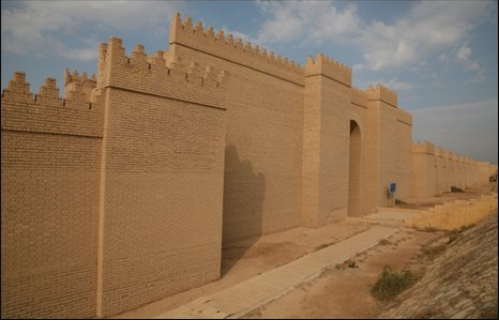
\includegraphics[width=.9\linewidth]{./img/WallsBabylon.png}
\caption{Wall of Babylon}
\end{figure}

Provides great security, allows for focus on other aspects of life.

\subsubsection{{\bfseries\sffamily TODO} Archimedes Screw: Verify location of possible garden's location with Driggers.}
\label{sec-3-8-2}
Some scholars believe that this was how the supposed \emph{handing gardens} were irrigated.
\begin{figure}[htb]
\centering
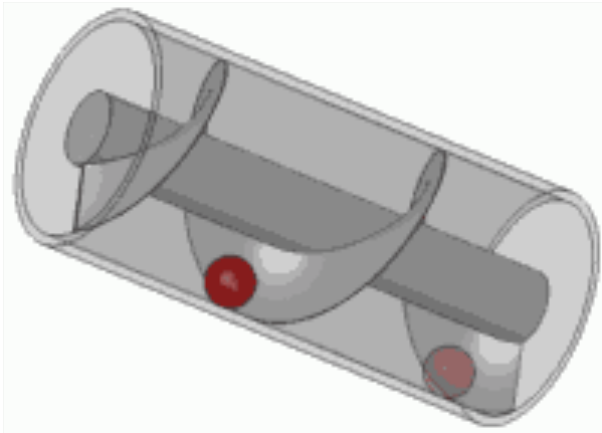
\includegraphics[width=.9\linewidth]{./img/archScrew.png}
\caption{Archimedes Screw}
\end{figure}

\begin{figure}[htb]
\centering
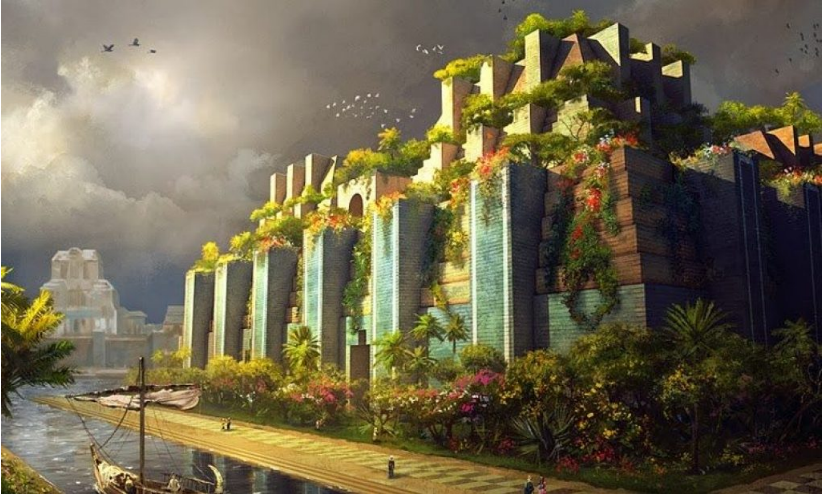
\includegraphics[width=.9\linewidth]{./img/HangingGardens.png}
\caption{Hanging Gardens}
\end{figure}

\begin{figure}[htb]
\centering
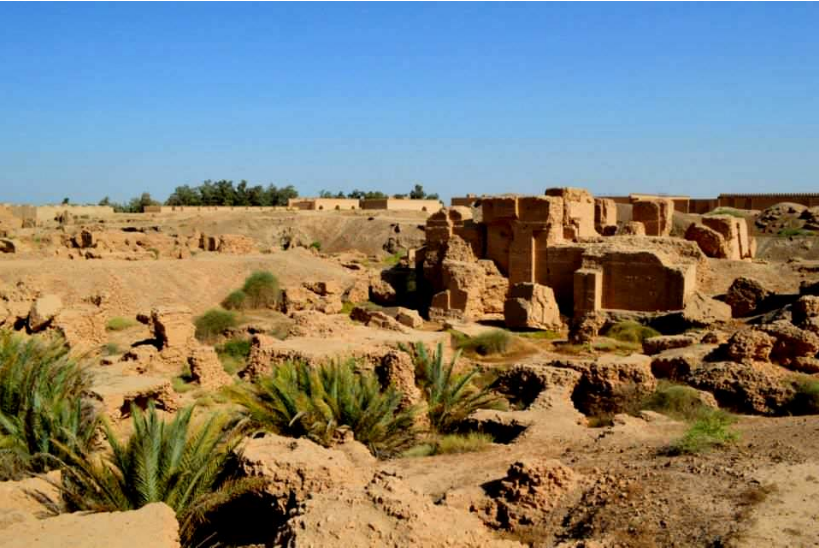
\includegraphics[width=.9\linewidth]{./img/HangingGardens2.png}
\caption{Possible location of gardens}
\end{figure}


\subsubsection{Assyrian Pottery}
\label{sec-3-8-3}
Allows travel to further distances away from immediate water access.

\subsubsection{Astronomy - Wrote down observations}
\label{sec-3-8-4}
This allows us to \emph{track} backwards in time and \emph{line up} our time line, and understandings with theirs.

\subsubsection{Mathematics}
\label{sec-3-8-5}
Mostly derived from needs of scribes, and clerks, doing tax calculations, record keeping was also important.

\begin{figure}[htb]
\centering
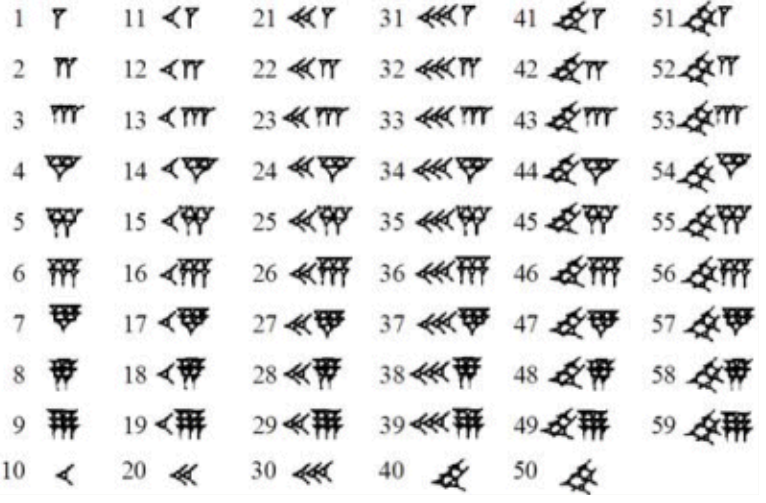
\includegraphics[width=.9\linewidth]{./img/CuneMath.png}
\caption{Cuneiform Mathematics symbols.}
\end{figure}

\begin{figure}[htb]
\centering
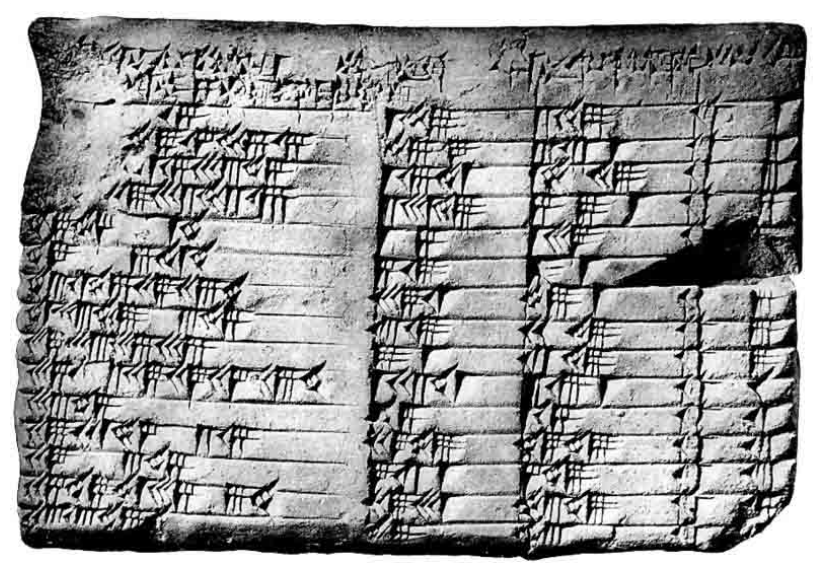
\includegraphics[width=.9\linewidth]{./img/acctRecs.png}
\caption{Accounting Records}
\end{figure}

\subsubsection{Medicine}
\label{sec-3-8-6}
\begin{figure}[htb]
\centering
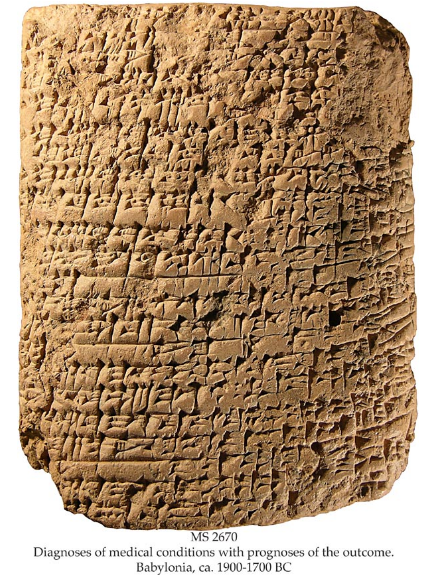
\includegraphics[width=.9\linewidth]{./img/MedRecs.png}
\caption{Medical Records}
\end{figure}

Scholars of early medicine started taking \emph{notes} about what methods worked, and those that didn't


\section{{\bfseries\sffamily TODO} Lecture 3 Ancient Egypt: Finish updating this info.}
\label{sec-4}
:DATE: \textit{<2018-01-25 Thu>}

**Objectives
\begin{itemize}
\item Survey of science, medicine, and technology in Ancient Egypt

\item Begin out exploration of the three subjects, mention above in world cultures

\item Briefly discuss \emph{Time}
\end{itemize}

\subsection{Opening Vignette}
\label{sec-4-1}
I have a Mining region of the sovereign
I had gown down to the sea
In a board 120 cubits long
40 cubits broad
in which there were 120 sailors for the choicest of Egypt\ldots{}
before it came they could fortell a gale
a storm before it existed

From A Tale of the Shipwrecked Sailor (Maybe from 2500 BC)

\begin{itemize}
\item Know that person was fairly intelligent.
\end{itemize}

\section{{\bfseries\sffamily TODO} Lecture 4}
\label{sec-5}
:DATE: \textit{<2018-01-25 Thu>}

\section{{\bfseries\sffamily TODO} Lecture 5}
\label{sec-6}
:DATE: \textit{<2018-02-01 Thu>}

\section{{\bfseries\sffamily TODO} Lecture 6 - Europe in the Middle Ages; Natural Philosophy: Remind driggers about quadrium}
\label{sec-7}
:Date: \textit{<2018-02-06 Tue>}

\subsection{middle ages}
\label{sec-7-1}
Two contributions medieval west gives us is Universities, and cathedrals
:EXAM: \textit{<2018-02-15 Tue>}

Driggers Dressed in grad robes.\\
\begin{itemize}
\item Hat like what was worn
\begin{itemize}
\item used to collect money after each lecture \texttt{approximately \$20}
\end{itemize}

\item Robe like Geneva rode, similar to priests
\item Colors represent
\end{itemize}

\texttt{Masters means to teach, or read}\\
Mace of university symbolic of power, president wears medallion to illustrate his power.\\

Oxford and Cambridge don't give out paper, they give out a \texttt{metaphysical} degree, they place hands on the graduate.\\
Doctorate comes from medieval period.\\
Coat of arms comes from this era also.\\

\begin{itemize}
\item Back rows similar to today's lectures.
\end{itemize}

\subsection{Introduction}
\label{sec-7-2}
5th - 15th century \\
\begin{itemize}
\item philosophy
\item medicine
\item soci
\item education in europe
\end{itemize}

\subsection{Timeline}
\label{sec-7-3}
[[]]
Organized this way because we look back, and organize history.//
Historians place order due to trends, sometimes they get it wrong.\\
During this time in Europe when bad things: wars, plagues - Golden age of Islam\ldots{}

\begin{itemize}
\item Collapse of W. Rome (372-410 CE)\\
\item Early middle ages (5th to 10th Century? CE)\\
\item High Middle ages (1001-1300 CE) \\
\end{itemize}
Renascence
\begin{itemize}
\item Late middle ages (1301-1500? CE)\\
\end{itemize}


As Islamic civilization continued golden age, they have more emirates, one in Spain.\\
Charlemagne main grandchild of person who stops advance of \emph{moores} 

byzantine empire expands\\
Western Europe has de urbanization problems, city governments abandoned.
\ldots{} Russians start to get organized

\subsection{Medieval Times}
\label{sec-7-4}
\begin{itemize}
\item social order\\
\item towns/urban spaces like\\
\item religious life and science?\\
\item Scientific production of med uro.
\end{itemize}

During this time in Europe when bad things: wars, plagues - Golden age of Islam\ldots{}
due to trends, sometimes they get it wrong.\\
\subsubsection{Zombie Apocalypse}
\label{sec-7-4-1}
What would happen if we had to abandon the city, where would we go? \\
Go to manors and agree to work in exchange for essentially \texttt{food}

\subsubsection{Feudalism}
\label{sec-7-4-2}
We don't really know where feudalism started. Most think England, maybe w. France.
\begin{itemize}
\item \textbf{Nobles} - highest is king - Obligated to defend other two groups \uline{can become \emph{knight groups}} \\
\item \textbf{Priests} - Praying for everyone all the time. ?Pray for people who might be in purgatory?
\item \textbf{Serfs} - People doing the work.
\end{itemize}

\subsection{Scholarly life}
\label{sec-7-5}
1050 and the return of "classical learning"\\
The importance of Aristotle v. Plato in Medieval Europe\\
\begin{itemize}
\item Aristotle most important, however, Plato was taught\ldots{}?\\
\item What is neo-platonism?\\
        Plato was very abstract and hard to translate.
$\backslash$\Some would say Jesus was a neo-platonist
\end{itemize}
\texttt{If western translators had done more of Plato's works the chances are good that we would see more of his works in this time period}
\begin{itemize}
\item Medieval Universities
\begin{itemize}
\item Curriculum and instruction\\
    Materials/ideas: 7 labors
\begin{itemize}
\item trivium help make an argument rhetoric type instruction. You know enough to go on.
\item quadrium
\end{itemize}
\item Scholasticism
\begin{itemize}
\item knowledge is publishing papers.
dismutation, debate around an issue - the nature of something.
\item More of a method than anything.
\end{itemize}
\end{itemize}
\end{itemize}

\subsubsection{Roger bacon}
\label{sec-7-5-1}
Medieval professor - forms basis of scientific method. Makes artificial rainbow and freaks out students.

\subsubsection{William of Ockham - Ockham's razor.}
\label{sec-7-5-2}

\subsubsection{Albert Magnus \emph{Albert the great}}
\label{sec-7-5-3}
Falconry regarded as scholar priest and professor


\subsubsection{Hildegard of Bingen Nun}
\label{sec-7-5-4}
Outlier example of intellectual thought done by women\\
\begin{itemize}
\item Creates a lot of music \emph{like a Renascence women}
\item Has a medical garden
\item publishes medical material
\end{itemize}

\subsubsection{Cristine Depuzon?}
\label{sec-7-5-5}
Wrote book about all women city state


\subsubsection{Thomas Aquinas}
\label{sec-7-5-6}
\begin{itemize}
\item Explains how different substances come to together to form new material.
\item Aquinas Cosmos
\begin{itemize}
\item Dante's inferno arises from this.
\end{itemize}
\end{itemize}
\subsection{Medieval engineering}
\label{sec-7-6}
\begin{itemize}
\item Heavy plows
\item Trebuchets
\item crossbow
\item could think of castles
\item Artificial power - wind mills
\end{itemize}

\subsection{Music}
\label{sec-7-7}
hurdi gurdi???

\subsection{Medieval medicine}
\label{sec-7-8}
\begin{itemize}
\item Black Death
\begin{itemize}
\item Some people think this was an oldschool ebola 
Sutonic virus
\end{itemize}
\end{itemize}
\subsubsection{Old theory}
\label{sec-7-8-1}
Rats on ships is how the diseases spread.
\begin{itemize}
\item Physicians and the plague
\end{itemize}



\begin{itemize}
\item Thought maybe astrological upsets caused the plagues.\\
\item serfs were able to negotiate for higher pay since soo many people died, there weren't many people around to work.\\
\end{itemize}
+Chronicles of the plague

\section{{\bfseries\sffamily TODO} Lecture  - test bank, Golden age of Islamic philosophy: email driggers about magic early Tuesday morning.}
\label{sec-8}
:DATE: \textit{<2018-02-08 Thu>}

\subsection{What to expect on test.}
\label{sec-8-1}
40*2 = 80\%
\begin{itemize}
\item m.c.
\item T/F, if a little false, all the way false\ldots{}
\item Fill in the blank
\end{itemize}
1 essay @ 20 pt
\begin{itemize}
\item Args
\item 3 \textbf{P} min
\item be detailed
\item Don't care about grammar for test essay.
\end{itemize}

\subsection{Outline}
\label{sec-8-2}
\begin{itemize}
\item historical case study
\item transition to byzantine empirer
\item \ldots{}
\end{itemize}

\subsection{Contextualizing Historical Terms}
\label{sec-8-3}
\begin{itemize}
\item Ancient Greek (500 - 336 BC)\\
\item Golden Age of Islmaic philosophy (\textasciitilde{} 700CE-1300 BCE)\\
\item The renaissance of eastern and wester Europe()\\
\end{itemize}

\subsection{Islamic era maps 1}
\label{sec-8-4}
Islamic era began after mohammed.

High era really ended after conquestor moved in (1497)???

Battle of toors charles montel stops military campain of moors\ldots{}

Mongols are busy during this time, Baghdad sacked during this time.

\subsection{Islamic era map 2}
\label{sec-8-5}
arrested dev of middle Europe?

\subsection{Scientific terms}
\label{sec-8-6}

\subsection{Cities of golden age}
\label{sec-8-7}
\begin{itemize}
\item Irrigation and Prosperity//
\item Relative city pops: really high
\end{itemize}

\subsection{Hydraulic Tech - The qanat}
\label{sec-8-8}
\begin{itemize}
\item Gently sloping tunnels, moves water from natural aquifers.
\item These had dams
\end{itemize}

\subsection{Transmission of tech}
\label{sec-8-9}
\begin{itemize}
\item Literate society\\
  This was due to the expectation of each individual reading the quaran every day.

\item Many uses of scientific instruments
\begin{itemize}
\item Case of astrolabe
\end{itemize}
\end{itemize}

Astrolabe can do over 300 types of calculations.
\begin{itemize}
\item Used to calculate direction of Mecca
\item Used to determine time of prayer.
\end{itemize}

Greeks/someone used to forecast horoscopes.

\subsection{Houses of wisdom}
\label{sec-8-10}
Literal translation factories in city of Baghdad
\begin{itemize}
\item Receive patronage from rulers of city\\
\item Functioned as library for person consumption, although typically he would allow other scholars access.
\end{itemize}

Also has intellectual effect
\begin{itemize}
\item While working on Greek translators, these translators come up with idea of science and other Greek aspects make up base for \texttt{good} knowledge.
\end{itemize}

Able to translate Greek texts to their religious texts.

\subsection{Hunaynn ibn Ishaq (Latin Iohannities) \texttt{you/yoo knight us}}
\label{sec-8-11}
contributing member of Islamic society.\\
fluent in Greek Syriac ???

Translated Greek into Syriac and his family translated into Arabic.

\subsection{Avicenna - Ibin Sinda}
\label{sec-8-12}
\begin{itemize}
\item natural philosopher and a physician\\
\item wrote book of healing and cannon of medicine
\end{itemize}

comes from present day Iran, understood Aristotle very well.

Saves life of one of royals, allowed to access their library, spends rest of days reflecting on these Greek texts.

\subsubsection{Book of healing}
\label{sec-8-12-1}
11th century
\begin{itemize}
\item more of encyclopedia: why things are the way they are.//
\end{itemize}

Criticize and interpreted Aristotle and made writings on this. Also became his own authority.

\subsubsection{Canon of medicine}
\label{sec-8-12-2}
Synthesis of Greek medicine ideas, and folk Arabic medicine, also poems and thoughts on medicine.\\
has ideas about incorporating feelings into humors.

\textbf{Rose water} had healing power, or so thought.

Most middle westerners liked him, he sands down Aristotle

\subsection{Medicine/Biology and Images 2}
\label{sec-8-13}
How do you convey images of body, when you have prohibitions on that type of study of body, not allowed to capture essence of a person's body//

Stuff was written to appear as words and shapes.
\subsection{}
\label{sec-8-14}
No structure\ldots{} Developed trig algebra, our numerals

\subsection{Mosque}
\label{sec-8-15}
Facilitated learning 
\subsection{observatories}
\label{sec-8-16}

\subsection{Midrasas? - law centers}
\label{sec-8-17}


\subsection{{\bfseries\sffamily TODO} Hospitals: The medieval Islamic hospital \texttt{in lib}}
\label{sec-8-18}
Christian physicians were astonished to see female healers.

\subsection{Toledo, Spain}
\label{sec-8-19}
Man religions worked together on translations

Archbishop was able to get scholars of different backgrounds to work together.

\textbf{reconquist} redefines boundaries of Islamic society.
\begin{itemize}
\item After this a lot of the texts are left behind, and invading peoples rediscover the ancient Greek texts.
\end{itemize}

\textbf{Erasure of middle eastern contribution to science from Islamic society}

\subsection{Byzantine empire - Byzantium 2}
\label{sec-8-20}
Mostly spoke Greek here.//
new streams of Latin development

Roman Catholic Church uses Latin

Orthodox church use Greek

Byz's loved horse races, like today's football.

\subsection{Crusades have huge affects, we don't really get into it\ldots{}..yet.}
\label{sec-8-21}
% Emacs 25.3.1 (Org mode 8.2.10)
\end{document}
